In questo capitolo discuteremo della qualità dei dati contenuti nei dataset utilizzati prima e dopo il processo di integrazione; inoltre, proporremo delle analisi descrittive effettuate sui dati integrati. 
\section{Descrizione dei dataset}
I 3 dataset utilizzati, che sono presenti nella \href{https://gitlab.com/Daniele-Papetti/kickstarterprediction}{repository online}, sono stati scaricati dal sito \href{https://www.kaggle.com/}{\emph{www.kaggle.com/}}.
In particolare, due di questi dataset (\textit{countries of the world.csv} e \textit{ks-projects-201612.csv}) sono quelli che verrano utilizzati effettivamente per estrarre delle \textit{features} per il processo di apprendimento automatico, mentre il terzo (\textit{country\_code.csv}) viene utilizzato sia come dizionario per l'analisi di qualità dei dati, sia per la parte di integrazione.\\
Il dataset \textit{countries of the world.csv} contiene informazioni che descrivono il rispettivo territorio e sviluppo di 227 nazioni del mondo; si veda la Tabella \ref{tab:world_countires_att} per i dettagli.
\begin{table}
	\caption{Tabella riassuntiva degli attributi presenti nel file \textit{countries of the world.csv}.\\(*) Si veda la Sotto sezione \ref{subsec:temporali}.}

	\label{tab:world_countires_att}

	\centering
	\begin{tabular}{|c|c|c|}
		\hline
		\textbf{Nome attributo} & \textbf{Tipo di dato} & \textbf{Descrizione} \\ 
		\hline  
		\rule{0pt}{13pt}\emph{Country} & Stringa & Nome della nazione \\ 
		\hline  
		\rule{0pt}{24pt}Region & Stringa & \shortstack{Regione del mondo \\ in cui è situata la nazione} \\ 
		\hline  
		\rule{0pt}{13pt}Population & Intero & Numero di abitanti in quella regione \\ 
		\hline  
		\rule{0pt}{24pt}Area & Intero & \shortstack{Estensione in miglia al quadrato \\ della superficie della nazione} \\ 
		\hline   
		\rule{0pt}{24pt}Pop. Density & \shortstack{Numero con \\ virgola mobile} & Numero di abitanti per miglio quadro \\ 
		\hline   
		\rule{0pt}{24pt}Coastline & \shortstack{Numero con \\ virgola mobile} & \shortstack{Rapporto tra area costiera \\ e area non costiera (*)} \\ 
		\hline   
		\rule{0pt}{24pt}Net migration & \shortstack{Numero con \\ virgola mobile} & Tasso di migrazione netta \\ 
		\hline  
		\rule{0pt}{24pt}Infant mortality & \shortstack{Numero con \\ virgola mobile} & Mortalità infantile ogni 1000 nascite \\ 
		\hline  
		\rule{0pt}{13pt}GDP & Intero & PIL \textit{pro capite} \\ 
		\hline  
		\rule{0pt}{24pt}Literacy & \shortstack{Numero con \\ virgola mobile} & Percentuale di alfabetismo \\ 
		\hline  
		\rule{0pt}{24pt}Phones & \shortstack{Numero con \\ virgola mobile} & Numero di telefoni ogni 1000 persone \\ 
		\hline  
		\rule{0pt}{24pt}Arable & \shortstack{Numero con \\ virgola mobile} & Percentuale di terreno arabile \\ 
		\hline  
		\rule{0pt}{24pt}Crops & \shortstack{Numero con \\ virgola mobile} & Percentuale di terreno coltivato \\ 
		\hline  
		\rule{0pt}{24pt}Other & \shortstack{Numero con \\ virgola mobile} & \shortstack{Percentuale di terreno che non\\ ricade nelle due categorie precedenti} \\ 
		\hline  
		\rule{0pt}{24pt}Climate & \shortstack{Numero con \\ virgola mobile} & \shortstack{Clima nella nazione, \\ i numeri sono associati ad un relativo clima}  \\ 
		\hline  
		\rule{0pt}{24pt}Birthrate & \shortstack{Numero con \\ virgola mobile} & Tasso di natalità \\ 
		\hline  
		\rule{0pt}{24pt}Deathrate & \shortstack{Numero con \\ virgola mobile} & Tasso di mortalità \\ 
		\hline  
		\rule{0pt}{24pt}Agriculture & \shortstack{Numero con \\ virgola mobile} & \shortstack{Percentuale di diffusione \\ del settore primario} \\ 
		\hline  
		\rule{0pt}{24pt}Industry & \shortstack{Numero con \\ virgola mobile} & \shortstack{Percentuale di diffusione \\ del settore secondario} \\ 
		\hline   
		\rule{0pt}{24pt}Service & \shortstack{Numero con \\ virgola mobile} & \shortstack{Percentuale di diffusione \\ del settore terziario} \\ 
		\hline  
	\end{tabular}
\end{table} 
%Tra queste si possono trovare informazioni utili come il PIL (GDP) \textit{pro capite}, lo sviluppo in percentuale dei tre settori ed il numero medio di telefoni per abitante; la chiave della relazione è il nome della nazione per esteso.
Invece, \textit{ks-projects-201612.csv} è il dataset contenente tutte le informazioni riguardo i progetti kickstarter fino a Dicembre 2016, si tratta di più di 323 mila istanze; gli attributi del dataset sono riportati nella Tabella \ref{tab:ks}.
\begin{table}
	\caption{Tabella riassuntiva degli attributi presenti nel file \textit{ks-projects-201612.csv}.}
	
	\label{tab:ks}
	
	\centering
	\begin{tabular}{|c|c|c|}
		\hline
		\textbf{Nome attributo} & \textbf{Tipo di dato} & \textbf{Descrizione} \\ 
		\hline  
		\rule{0pt}{13pt}\emph{ID} & Intero & ID interno di kickstarter \\ 
		\hline  
		\rule{0pt}{13pt}Name & Stringa & Nome del progetto \\ 
		\hline  
		\rule{0pt}{13pt}Category & Stringa & Categoria specfica del progetto \\ 
		\hline  
		\rule{0pt}{24pt}Main category & Stringa & \shortstack{Categoria più generica \\ in cui ricade il progetto} \\ 
		\hline   
		\rule{0pt}{24pt}Currency & Stringa & \shortstack{Valuta monetaria usata \\ per supportare il progetto} \\ 
		\hline   
		\rule{0pt}{13pt}Deadline & Data & Data di termine campagna \\ 
		\hline   
		\rule{0pt}{24pt}Goal & Intero & \shortstack{Ammontare monetario da venir raggiunto \\ purché si possa realizzare il progetto} \\ 
		\hline  
		\rule{0pt}{13pt}Launched & Data & Data di lancio della campagna \\ 
		\hline  
		\rule{0pt}{24pt}Pledged & \shortstack{Numero con \\ virgola mobile} & Ammontare monetario donato \\ 
		\hline  
		\rule{0pt}{13pt}State & Stringa & Stato del progetto \\ 
		\hline  
		\rule{0pt}{24pt}Backers & Intero & \shortstack{Numero di persone che hanno \\ supportato la campagna} \\ 
		\hline  
		\rule{0pt}{24pt}Country & Stringa & \shortstack{Codice della nazione in cui \\ è stata avviata la campagna} \\ 
		\hline  
		\rule{0pt}{24pt}Usd pledged & \shortstack{Numero con \\ virgola mobile} & Corrispetti in dollari americani donati \\ 
		\hline
	\end{tabular}
\end{table} 
Poiché i due dataset devono venire fusi mediante le nazioni, le quali però sono rappresentate in modo differente (il primo ha il nome completo delle nazioni ed il secondo il codice a due caratteri), abbiamo dovuto utilizzare un terzo dataset (\textit{country\_code.csv}) che mettesse in relazione i nomi delle nazioni ed il loro codice, in totale sono conenute le informazioni riguardo 247 nazioni; si faccia riferimento alla Tabella \ref{tab:code} per la semantica della relazione.

\begin{table}
	\caption{Tabella riassuntiva degli attributi presenti nel file \textit{country\_code.csv}.}
	
	\label{tab:code}
	
	\centering
	\begin{tabular}{|c|c|c|}
		\hline
		\textbf{Nome attributo} & \textbf{Tipo di dato} & \textbf{Descrizione} \\ 
		\hline  
		\rule{0pt}{13pt}\emph{ID} & Intero & ID incrementale \\ 
		\hline  
		\rule{0pt}{13pt}Country name & Stringa & Nome della nazione \\ 
		\hline  
		\rule{0pt}{13pt}Code 2digit & Stringa & Codice di due cifre univoco \\ 
		\hline  
		\rule{0pt}{13pt}Code 3digit & Stringa & Codice di tre cifre univoco \\ 
		\hline   
	\end{tabular}
\end{table} 

\section{Analisi di qualità dei dataset (pre-integrazione)}
In questa sezione verranno presentate tutte le misure di qualità effettuate sui singoli dataset prima del processo di integrazione.
I dataset analizzati, come già detto, sono i due dataset da cui poi verranno estratte le \textit{features}: \textit{countries of the world} e \textit{ks-projects-201612}.
Per quanto concerne \textit{countries of the world} sono state effettuate le seguenti misure:
\begin{itemize}
	\item accuratezza sintattica rispetto all'attributo Country;
	\item misure di completezza rispetto a tutti gli attributti.
\end{itemize}
Al contempo, \textit{ks-projects-201612} è stato analizzato rispetto alle seguenti metriche:
\begin{itemize}
	\item accuratezza sintattica rispetto ai codici delle nazioni;
	\item indagine dei valori assunti dall'attributo State;
	\item consistenza dell'attributo State;
	\item consistenza dell'attributo Backers;
	\item misure di completezza rispetto a tutti gli attributi.
\end{itemize}
Infine, per ambo i dataset sono stati valutati anche la temporalità e la leggibilità.

\subsection{Accuratezza sintattica dell'attributo Country del dataset delle nazioni}
Come detto in precedenza, per misurare l'accuratezza sintattica rispetto all'attributo Country del dataset contenente le informazioni sulle nazioni è stato utilizzato un secondo dataset come dizionario.
In prima battuta, abbiamo cercato dei match perfetti tra i nomi delle nazioni, ovvero le coppie di stringhe la cui distanza di edit è pari a zero.
Per tutti i casi in cui non è stato possibile individuare un match perfetto, si è in primo luogo provato ad aumentare la soglia di distanza di edit, ottenendo però scarsi risultati.
Il motivo di ciò è dovuto al fatto che i non match spesso sono causati da modi diversi di riferirsi ad una stessa nazione (\textit{i.e.}, Vietnam e Viet Nam) o la presenza di un prefisso davanti al nome con cui normalmente ci si rifersce alla nazione (\textit{i.e.}, The Bahamas e Bahamas).
A fronte di ciò, si è deciso di utilizzare una distanza basata sulle Bigram in modo da ridurre problemi causati dalle situazioni descritte in precedenza; gli intervalli per cui stabilire se si sono ottenuti dei match, non match o dubbio sono state rispettivamente: $[0.7, 1.0], [0.0,0.5], (0.5, 0.7)$, si faccia riferimento alla Tabella \ref{tab:matches} per i dettagli.
Poiché in tutti 3 i casi le tuple sono di un numero molto ridotto si è deciso ulteriormente di verificare “a mano” dei possibili falsi positivi o negativi, oltre a risolvere a mano le situazioni di dubbio.
Dall'analisi effettuata, siamo arrivati a stabilire l'assenza di falsi positivi e la presenza di 4 falsi positivi (ovvero il 36 \%, si ricorda che in totale sono stati riscontrati 11 non match), per le situazioni di dubbio sono stati trovati 7 match ed un solo non match.
A fronte di questi numeri, si possono fare ulteriori considerazioni a posteriori per quanto concerne la determinazione delle soglie abbassando il limite superiore della soglia di dubbio e dei non match, ottenendo così delle distribuzioni di errori più ragionevoli. 
Poiché il dominio applicativo, in questo caso, è costituito da un dataset molto ristretto, tali conflitti possono essere risolti “a mano” senza dover modificare le soglie e rianalizzare la distribuzione degli errori. 
Quest'analisi è stata poi utilizzata per modificare il dataset contenente le nazioni e i relativi codici in modo da aver un dataset accurato per le attività di integrazione.\\
In Figura \ref{fig:dqcountrycodeaccuracy} è presente la pipeline utilizzata in Pentaho per l'analisi di questa metrica.
\todo[inline]{Figura Errata! serve quella del primo pezzo del file data\_quality DP}
\begin{table}
	\caption{Tabella riassuntiva contenente numero e percentuale (si ricorda che si hanno 227 nazioni) dei match perfetti e match, non match e dubbio secondo le bigram calcolate sulle nazioni che non hanno avuto il match perfetto.}
	
	\label{tab:matches}
	
	\centering
	\begin{tabular}{|c|c|c|}
		\hline
		 & \textbf{Numero} & \textbf{Percentuale (\%)} \\ 
		\hline  
		\rule{0pt}{13pt}Match perfetti & 188 & 83 \\ 
		\hline  
		\rule{0pt}{13pt}Match & 20 & 9 \\ 
		\hline  
		\rule{0pt}{13pt}Non match & 11 & 5 \\ 
		\hline  
		\rule{0pt}{13pt}Dubbio & 8 & 3 \\ 
		\hline   
	\end{tabular}
\end{table} 

\begin{figure}[h!]
	\centering
	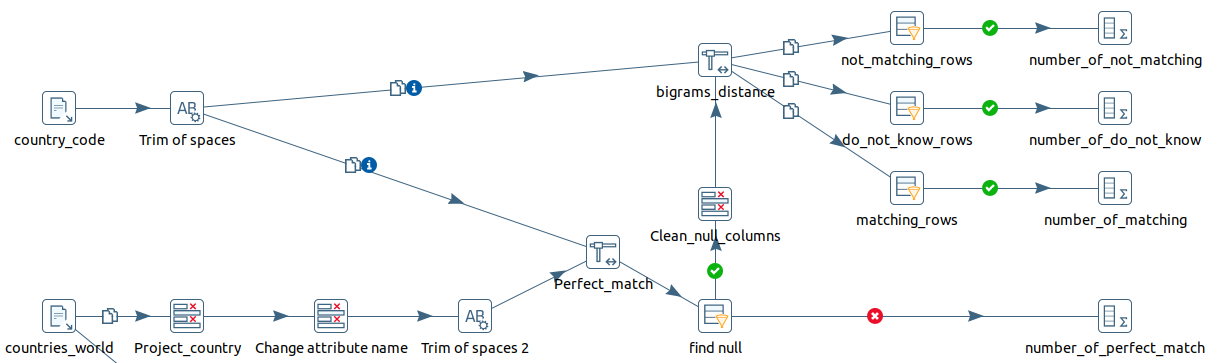
\includegraphics[width=0.7\linewidth]{images/DQ_countrycodeaccuracy}
	\caption{Pipeline per il conteggio delle tuple con codice della country non valido.}
	\label{fig:dqcountrycodeaccuracy}
\end{figure}

\subsection{Completezza del dataset delle nazioni}
La completezza analizzata è la completezza per attributo, in particolare abbiamo utilizzato la definizione “standard”, ovvero:\\“il numero di valori  \texttt{null} che compaiono nella colonna di un attributo.”\\
Stando alla definizione, non abbiamo ricercato possibili valori non \texttt{null} ma i quali non possegono valori semantici corretti rispetto all'attributo.
Questa casistica è stata analizzata e studiata per la parte di integrazione dei dati ma non per la parte di completezza, poiché ci siamo limitati alla definizione di completezza. 
In Tabella \ref{tab:compl_country} sono presenti il numero e la relativa percentuale di valori \texttt{null} per ogni colonna, infine si è contato anche il numero complessivo di valori nulli e la loro percentuale rispetto al totale dei valori.
Dalle misure effettuate, possiamo dire che il dataset è praticamente completo, soprattutto riguardo al GDP che è un attributo che verrà utilizzato per la parte di apprendimento automatico.
\begin{table}
	\caption{Tabella riassuntiva contenente numero e percentuale (si ricorda che si hanno 227 nazioni) dei \texttt{null} presenti nel dataset per ogni attributo. Infine, si fornisce un'ultima riga contenente il numero totale di \texttt{null} e la percentuale rispetto ad ogni campo del dataset.}
	
	\label{tab:compl_country}
	
	\centering
	\begin{tabular}{|c|c|c|}
		\hline
		\textbf{Attributo}  & \textbf{Numero} & \textbf{Percentuale (\%)} \\ 
		\hline  
		\rule{0pt}{13pt}Country & 0 & 0 \\ 
		\hline  
		\rule{0pt}{13pt}Region & 0  & 0 \\ 
		\hline  
		\rule{0pt}{13pt}Population & 0 & 0 \\ 
		\hline  
		\rule{0pt}{13pt}Area & 0 & 3 \\ 
		\hline
		\rule{0pt}{13pt}Pop. Density & 0 & 0 \\
		\hline
		\rule{0pt}{13pt}Coastline & 0 & 0 \\
		\hline
		\rule{0pt}{13pt}Net migration & 3 & 1 \\
		\hline
		\rule{0pt}{13pt}Infant mortality & 3 & 1 \\
		\hline
		\rule{0pt}{13pt}GDP & 1 & 0.4 \\
		\hline
		\rule{0pt}{13pt}Literacy & 18 & 8 \\
		\hline
		\rule{0pt}{13pt}Phones & 4 & 2 \\
		\hline
		\rule{0pt}{13pt}Arable & 2 & 1 \\
		\hline
		\rule{0pt}{13pt}Crops & 2 & 1 \\
		\hline
		\rule{0pt}{13pt}Other & 2 & 1 \\
		\hline
		\rule{0pt}{13pt}Climate & 22 & 10 \\
		\hline
		\rule{0pt}{13pt}Birthrate & 3 & 1 \\
		\hline
		\rule{0pt}{13pt}Deathrate & 4 & 2 \\
		\hline
		\rule{0pt}{13pt}Agriculture & 15 & 7 \\
		\hline
		\rule{0pt}{13pt}Industry & 16 & 7 \\
		\hline
		\rule{0pt}{13pt}Service & 15 & 7 \\
		\hline   
		\rule{0pt}{13pt}\textbf{Totale} & \textbf{110} & \textbf{2.4} \\
		\hline
	\end{tabular}
\end{table}

\todo[inline]{Ricordarsi di mettere poi il riferimento alla figura DP}
\todo[inline]{Pipeline della completezza di world country DP}

\subsection{Accuratezza sintattica del codice delle nazioni del dataset Kickstarter}


\subsection{Accuratezza sintattica attributo state (Figura \ref{fig:dqstateaccuracy})}

\begin{figure}[h!]
	\centering
	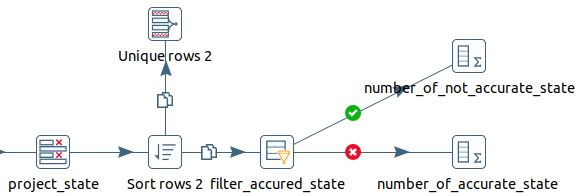
\includegraphics[width=0.7\linewidth]{images/DQ_stateaccuracy}
	\caption{Pipeline che verifica tutti i possibili valori dell'attributo state. Gli unici valori plausibili e accettati dovrebbero essere successful, faild, cancelled, live e suspended.}
	\label{fig:dqstateaccuracy}
\end{figure}


\subsection{Consistenza attributo state (Figura \ref{fig:dqstateaconsistency})}

\begin{figure}[h!]
	\centering
	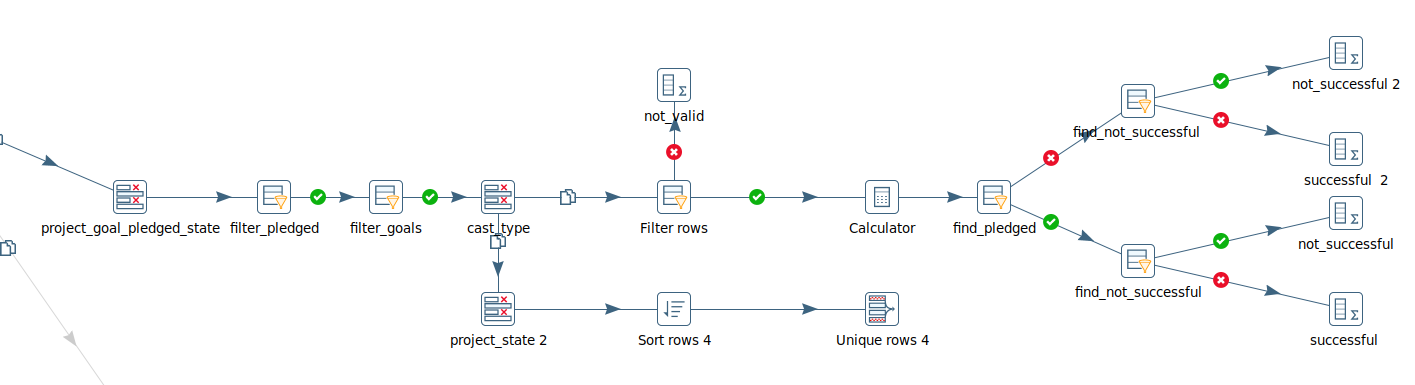
\includegraphics[width=0.7\linewidth]{images/DQ_stateaconsistency}
	\caption{Pipeline per il conteggio delle tuple il cui valore dell'attributo state non è consistente con il totale del denaro raccolto.}
	\label{fig:dqstateaconsistency}
\end{figure}


\subsection{Consistenza attributo backers (Figura \ref{fig:dqbackersconsistency})}

\begin{figure}[h!]
	\centering
	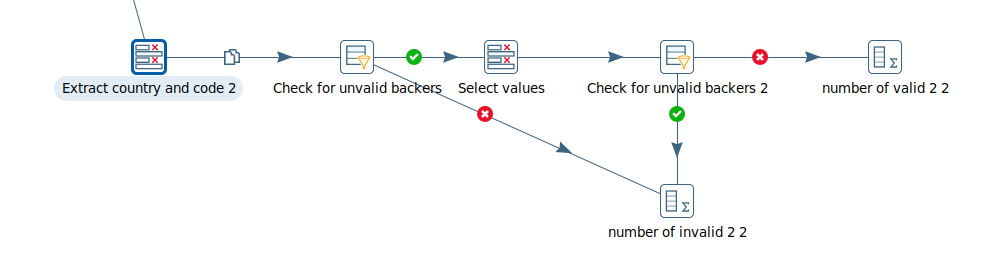
\includegraphics[width=0.7\linewidth]{images/DQ_backersconsistency}
	\caption{Pipeline per il conteggio delle tuple il cui valore dell'attributo backers assume un valore negativo oppure non è consistente con il totale del denaro raccolto.}
	\label{fig:dqbackersconsistency}
\end{figure}


\subsection{Completezza del dataset Kickstarter (Figura \ref{fig:dqcompletezza})}
\todo[inline]{tua parte}
La profilazione dei dati eseguita in precedenza ha mostrato possibili casi di valori sintatticamente corretti ma semanticamente errati; in particolare, un piccolo sottoinsieme di tuple (circa 500) ha mostrato valori privi di senso in diversi campi. Questo sottoinsieme di tuple è stato rimosso dalle operazioni di trasformazione eseguite successivamente, ed è quindi stato deciso di non includere il conteggio di queste tuple nell'analisi della completezza

\begin{figure}[h!]
	\centering
	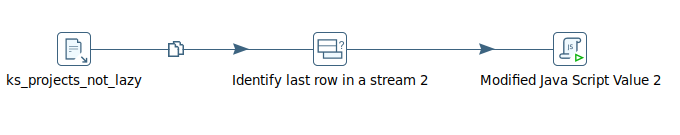
\includegraphics[width=0.7\linewidth]{images/DQ_completezza}
	\caption{Pipeline che utilizza uno script Javascript custom che itera sui campi del dataset e conta il numero di tuple con valore dell'attributo nullo.}
	\label{fig:dqcompletezza}
\end{figure}


\subsection{Accessibilità dei dataset}
Tutti i dataset analizzati mostrano un ottimo livello di accessibilità da parte dell'utente, con nomi degli attributi auto-esplicativi e facile reperibilità dei dati di interesse. 
Le uniche note a margine di quanto appena detto sono i valori dell'attributo \textit{Climate}, poiché sono dei numeri la cui semantica non è stata specificata, inoltre l'attributo \textit{Coastline} anche se intuitivo non è chiaro come sia stato calcolato, si è supposto essere il rapporto tra area costiera e non costiera, ma non si ha la certezza.
Per questo motivo, non si è resa necessaria la creazione di viste sugli schemi locali dei dataset, mantenendo inalterata la struttura di questi ultimi.

\subsection{Porprietà temporali}
\label{subsec:temporali}
Il dataset \textit{ks-projects-201612.csv} contiene tutti i progetti registrati sulla piattaforma Kickstarter fino alla fine del 2016. Il dataset \textit{countries of the world.csv} contiene invece statistiche sugli stati che si riferiscono all'anno 2017. Ne consegue che i dati non siano perfettamente coerenti dal punto di vista temporale, ma abbiamo reputato questo sfasamento marginale, considerata l'assenza di modifiche radicali degli indici statistici presi in considerazioni negli anni consecutivi.

\section{Processo di integrazione dei dati}
Al fine di produrre un dataset integrato per il processo di Machine Learning, si è reso necessario unire i tre dataset scelti in un unico schema integrato. Prima di fare ciò, sfruttando le considerazioni fatte nella parte di analisi di qualità dei dati, sono state eseguite una serie di operazioni di pulizia e raffinamento dei dati.\\

\begin{figure}
	\hspace*{-1cm}%
	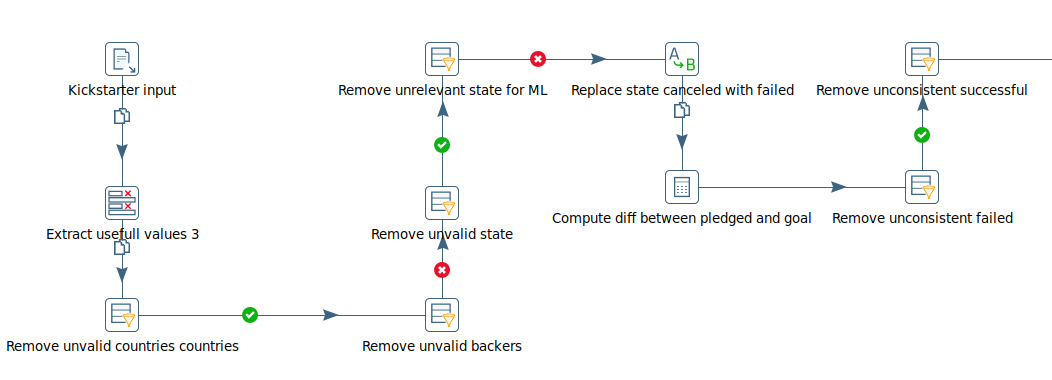
\includegraphics[width=\dimexpr\textwidth+2cm\relax]{images/transformation_kick}%
	\hspace*{-1cm}%
	\caption{Pipeline di trasformazione per il dataset contenente i dati dei progetti Kickstarter}
	\label{fig:transformationkick}
\end{figure}

\subsection{Dataset Kickstarter}
Inizialmente sono stati eliminati tutti quegli attributi che non avevano alcuna informazione rilevante ai fini del training del modello di Machine Learning (Data di creazione e di terminazione, nome, moneta utilizzata \dots).\\
In seguito sono stati rimossi tutti quei record il cui campo relativo alla nazione di origine violasse la rappresentazione standard, ovvero due lettere dell'alfabeto maiuscole. Ciò si è reso necessario in quanto l'analisi della accuratezza sintattica sul campo aveva mostrato una serie di valori privi di significato.\\
Sono stati poi rimossi una serie di record che creavano problemi di consistenza per quanto riguarda il campo dei sostenitori e del totale raccolto. Le analisi condotte in precedenza avevano infatti rilevato che alcuni record avevano un numero di sostenitori negativo, oppure un numero di sostenitori pari a zero, ma il campo che rappresenta l'ammontare del denaro raccolto non era zero anch'esso.\\
E' stata poi condotta una operazione di raffinazione sul campo \textit{state} del dataset, che rappresenta lo stato in cui il progetto si trova. Dopo aver rimosso tutti i valori sintatticamente privi di senso, abbiamo deciso di rimuovere tutti i record il cui stato fosse live, ovvero ancora in corso, oppure suspended, ovvero bloccati dalla piattaforma Kickstarter per violazioni dei termini contrattuali. Questa decisione è stata presa in quanto questo tipo di record potrebbe influenzare negativamente le performance del modello di Machine Learnig, fornendo tuple con uno stato di dubbio significato.
E' stato poi deciso di rendere tutti i record con il campo state uguale a canceled, ovvero cancellati dal creatore, come progetti falliti.\\
Infine, sono stati rimossi tutti i record che mostravano inconsistenza tra lo stato del progetto e la differenza tra denaro richiesto e denaro raccolto. E' infatti mandatorio che se è stato raccolto più denaro di quanto richiesto, il progetto risulti completato, mentre se non sono stati raccolti fondi sufficienti, il progetto risulti fallito.\\
L'intera pipeline di trasformazione è riportata in Figura \ref{fig:transformationkick}.


\subsection{Countries}
Siccome il dataset contenente i dettagli sui progetti Kickstarter sfrutta il codice di 2 lettere per rappresentare la nazione di origine del progetto, mentre il dataset con le informazioni circa il livello di sviluppo dei vari paesi sfrutta il nome completo, è stato necessario individuare un terzo dataset da utilizzare come una tabella di join, in modo da associare ogni nome per esteso con il relativo codice di due lettere.\\
Il dataset individuato per questo scopo si è però rivelato utilizzare una differente sintassi per rappresentare il nome per esteso dei paesi. Per questo motivo, sono state applicate delle tecniche di record linkage per individuare i record corrispondenti ed uniformare la sintassi di questi. Per fare ciò, sono stati utilizzati i dati prodotti dal processo di analisi di qualità dei dati (trattato nella prima parte di questo documento).\\
In particolare, sono stati ignorati i record di perfect match prodotti dalla distanza di edit con soglia zero, mentre sono stati confrontati caso per caso i risultati prodotti dall'analisi tramite bigram. Ponendo la soglia di match a 0.7 e la soglia di non match a 0.5, la soluzione proposta ha prodotto performance ottime, individuando correttamente tutti i match (20/20), e buona parte dei non match(7/11). La presenza di casi limite, quali rappresentazioni radicalmente diverse di un medesimo record, ha reso necessario la supervisione manuale per un piccolo sottoinsieme di questi record.\\

\begin{figure}
	\centering
	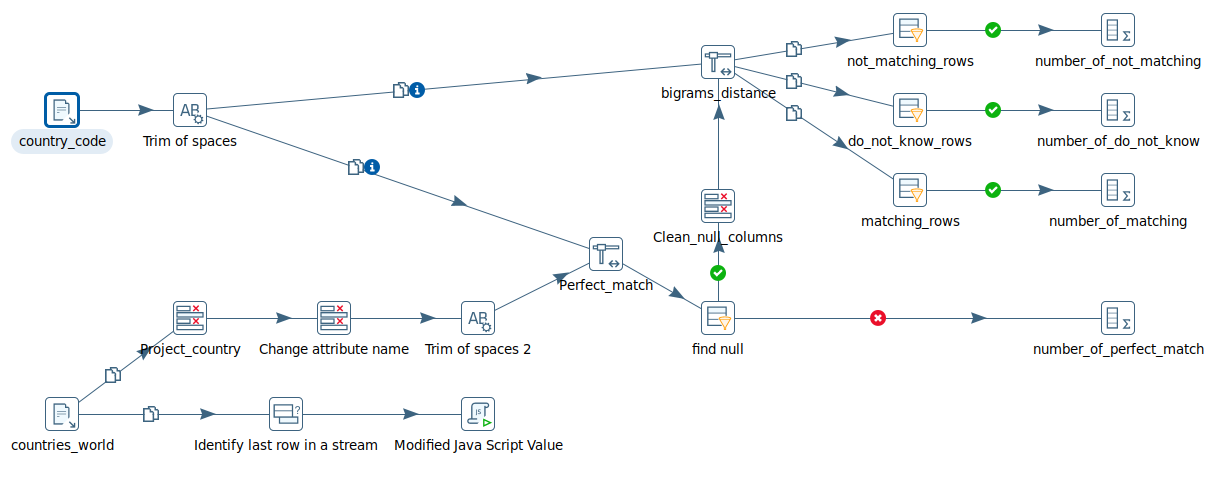
\includegraphics[width=0.7\linewidth]{images/RecordLinkage}
	\caption{Pipeline eseguita per realizzare le operazioni di record linkage}
	\label{fig:recordlinkage}
\end{figure}


\section{Produzione dataset integrato}
A seguito del processo di raffinamento e integrazione dei dataset esposto in precedenza, i tre database sono stati uniti in un unica tabella tramite delle operazioni di merge join, per motivi di efficienza.\\
A seguito dell'unione, sono stati prodotti due nuovi dataset (come mostrato in Figura \ref{fig:transformationcomplete}), uno contenente tutti gli attributi risultanti dalle operazioni precedenti, mentre l'altro epurato da tutti gli attributi privi di valore ai fini dell'addestramento del modello di Machine Learning.

\begin{figure}[p!]
	\centering
	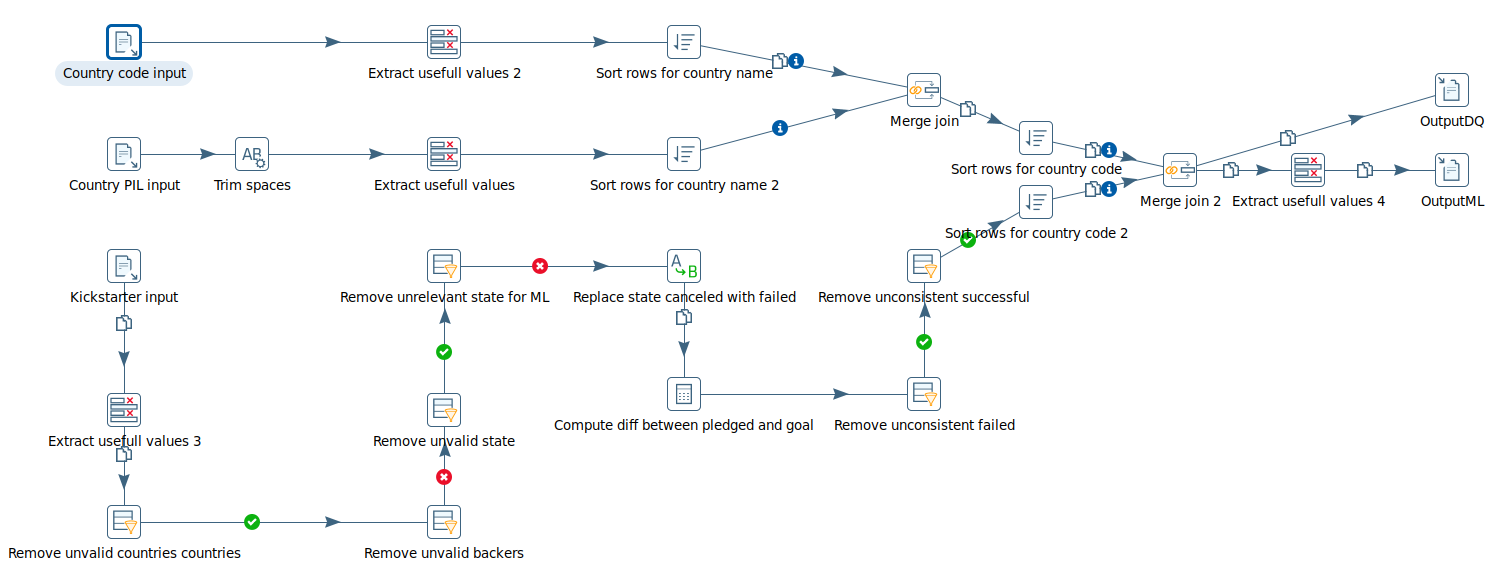
\includegraphics[angle=90,origin=c,width=0.55\linewidth]{images/transformation_complete}
	\caption{Pipeline di trasformazione per il dataset contenente i dati dei progetti Kickstarter}
	\label{fig:transformationcomplete}
\end{figure}

\newpage
\section{Analisi di qualità dei dataset (post-integrazione)}
Al fine di valutare la qualità del lavoro svolto nella fase di integrazione del dataset, le misure di qualità precedentemente stabilite sono state applicate al dataset integrato. In questa sezione verranno riportati i risultati ottenuti e relative considerazioni.

\subsection{Accuratezza sintattica attributo country (Figura \ref{fig:dqtcountries})}
L'attributo presenta 21 possibili valori, tutti formati da una coppia di 2 lettere maiuscole dell'alfabeto. Non sono presenti tuple con valore dell'attributo che violino questo vincolo sintattico.

\begin{figure}[h!]
	\centering
	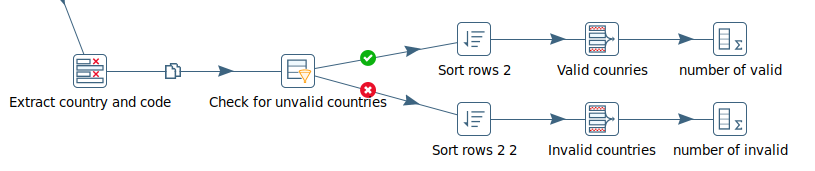
\includegraphics[width=1\linewidth]{images/DQT_countries}
	\caption{Pipeline per la verifica della accuratezza sintattica dell'attributo country}
	\label{fig:dqtcountries}
\end{figure}


\subsection{Accuratezza sintattica attributo state (Figura \ref{fig:dqtstate})}
L'attributo state risulta assumere due possibili valori, successful e failed. Le trasformazioni applicate producono quindi una riduzione dei possibili valori da 408 a 2 possibili valori.

\subsection{Consistenza attributo state (Figura \ref{fig:dqtstate})}
Per l'attributo in esame, non sono presenti tuple inconsistenti, ove il totale raccolto non sia consistente con lo stato del progetto.

\begin{figure}[h!]
	\centering
	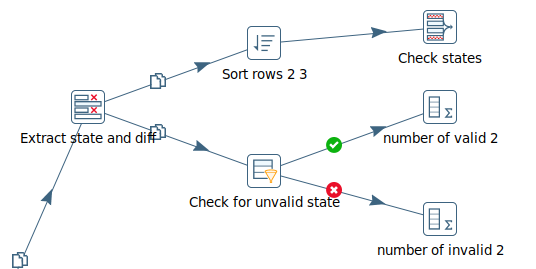
\includegraphics[width=0.6\linewidth]{images/DQT_state}
	\caption{Pipeline per la verifica della consistenza e della accuratezza sintattica dell'attributo state}
	\label{fig:dqtstate}
\end{figure}

\subsection{Consistenza attributo backers (Figura \ref{fig:dqtbackers})}
Per il campo backers, non sono state rilevate tuple con valore del campo negativo oppure con un valore non consistente con totale del denaro raccolto

\begin{figure}[h!]
	\centering
	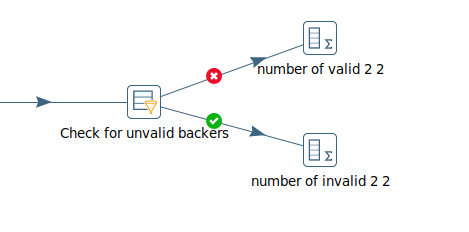
\includegraphics[width=0.7\linewidth]{images/DQT_backers}
	\caption{Pipeline per la verifica della consistenza dell'attributo backers}
	\label{fig:dqtbackers}
\end{figure}

\subsection{Completezza del dataset}
Ai fini di valutare la completezza del dataset prodotto, è stato eseguito nuovamente lo script che ricerca e conta i campi nulli presenti del dataset. L'esecuzione di questo processo conferma l'assenza di campi nulli nel dataset prodotto.

\subsection{Accessibilità del dataset}
Al fine di garantire una accessibilità ottimale al dataset sfruttato per eseguire il training del modello di Machine Learning, sono stati selezionati nomi significativi ed autoesplicativi per le gli attributi rappresentati nel dataset.

\subsection{Porprietà temporali}
Le considerazioni rimangono analoghe a quelle effettuate prima delle operazioni di integrazione dei dati.

\subsection{Altre misure di qualità}
Al fine di verificare l'efficacia dell'operazione di record linkage e data fusion (eseguite a mano) compiute sul campo country del dataset \textit{countries of the world.csv}, sono state nuovamente misurate le distanze con il campo country\_name del dataset \textit{country\_code.csv}. Questa misura, eseguita mediante la pipeline riportata in Figura \ref{fig:qdtrecordlinkage}, mostrano come il nome dei perfect match sia aumentato a seguito delle modifche apportate al dataset \textit{countries of the world.csv}. Allo stesso modo, sfruttando le bigrams, all'interno degli insiemi di incertezza e di non match, sono rimaste solo le coppie che effettivamente non dovevano essere linkate, mentre quelle rilevate come match nella prima analisi sono state tutte portate ad essere perfect match.

\begin{figure}[h!]
	\centering
	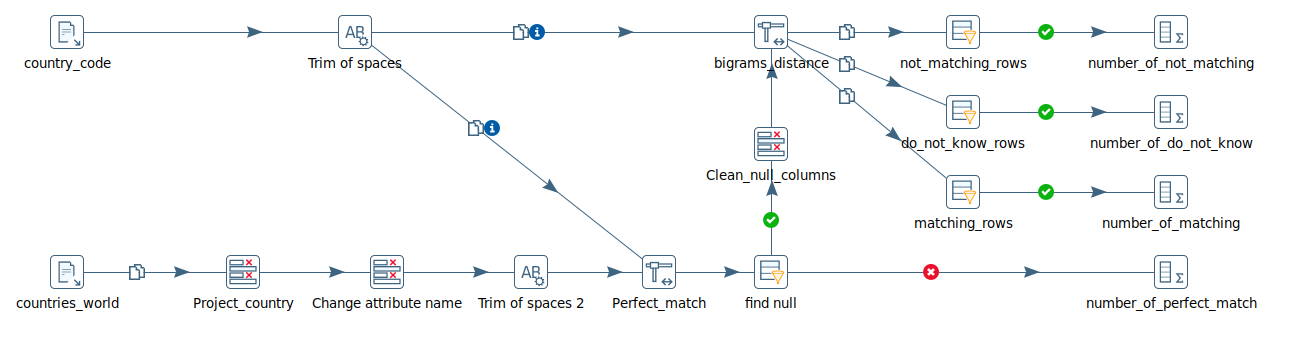
\includegraphics[width=1\linewidth]{images/QDT_recordlinkage}
	\caption{Pipeline utilizzata per la verifica del processo di record linkage effettuata}
	\label{fig:qdtrecordlinkage}
\end{figure}

\captionof{table}{Tabella riassuntiva che mostra il numero di tuple che non soddisfano i vincoli di consistenza o di accuratezza sintattica prima e dopo le trasformazioni applicate}

\begin{tabular}{|c|c|c|}
	\hline 
	Misura & Pre-trasformazione & Post-trasformazione \\ 
	\hline 
	Accuratezza sintattica state & 404 & 0 \\ 
	\hline 
	Consistenza state & 524 & 0 \\ 
	\hline 
	Accuratezza sintattica country code & 141 & 0 \\ 
	\hline 
	Consistenza backers & 3703 & 0 \\ 
	\hline 
	Completezza tabella & 3795 & 0 \\ 
	\hline 
\end{tabular} 

